\chapter{Concepts and Implementation of Conditional Random Field-based Semantic Segmentation}\label{ch:structured_pystruct}

Many classical computer vision applications such as stereo, optical flow, semantic
segmentation and visual grouping can be naturally formulated as image labeling tasks.
%
Arguably the most popular way to approach such labeling problems is via graphical
models, such as Markov random fields (MRFs) and conditional random fields (CRFs).
MRFs and CRFs provide a principled way of integrating local evidence and
modeling spacial dependencies, which are strong in most image-based tasks.
%
While in earlier approaches, model parameters were set by hand or using
cross-validation, more recently parameters are often learned using a max-margin
approach.

Most models employ linear energy functions of unary and pairwise interactions,
trained using structural support vector machines (SSVMs). While linear energy
functions lead to learning problems that are convex in the parameters, complex
constraints complicate their optimization. 

In recent years there has been a wealth of research in methods for learning
structured prediction, as well as in their application in areas such as natural
language processing and computer vision (see \citet{nowozin2011structured} for
an overview).
%
In this chapter, we will first introduce the concepts and algorithms used in
structured prediction, in particular in maximum margin methods. We will then
accompany this by a description of our open source implementation of these
algorithms, \pystruct.

\section{Basic Concepts in Structured Prediction}

Structured prediction can be defined as making a prediction $f(x)$ by maximizing a
compatibility function $g$ between an input $x$ and possible labels
$y$~\citep{nowozin2011structured}:
\begin{equation}
    f(x) = \argmax_{y \in \mathcal{Y}} g(x, y)
\end{equation}
The computation of $y$ in the above equation is often referred to as inference
or prediction.
While using arbitrary functions is possible, and was expored
in some recent works % TODO cite dtf, conditional neural fields
most current approaches use linear functions, leading to:
\begin{equation}\eqlabel{main_equation}
    f(x) = \argmax_{y \in \mathcal{Y}}\  \theta^T \Phi(x, y).
\end{equation}
Here, $y$ is a \emph{structured} label, $\Phi$ is a joint feature function of
$x$ and $y$, and $\theta$ are parameters of the model. \emph{Structured} means
that $y$ is more complicated than a single output class, for example a label
for each word in a sentence or a label for each pixel in an image.
Learning structured prediction means learning the parameters $\theta$ from training data.
The particular model that is used is completely encoded in $\Phi(x, y)$, which manifests
the relation between input $x$ and output $y$. As $\mathcal{Y}$ is typically very large,
it is crucial to exploit the particular form of $\Phi(x, y)$ to solve the inference problem
of \Eqref{main_equation}.

While $y$ could be a complicated like a parsing tree or the geometric
configuration of a molecule, many setting, such as the image segmentation
setting we are interested, can be reduced to the case where $y$ is a vector of
discrete labels $\mathcal{Y} = \{1, \dotsc, k\}^n$.
In the following, we will only discuss this multivatiate case. In general, $n$ is often different
for different inputs $x$, such as image with different number of (super) pixels.
We will ignore this in our notation to simplify the presentation.

\subsection{Factor Graphs and the Relation to Graphical Models}
% one factor graph per instance?
In the case when $y$ is multivariate, a very general and widely used method to
specify the structure of a model, and therefore $\Phi$, is using \emph{factor
graphs}. A factor graph is a bipartite graph $(\mathcal{V}, \mathcal{F},
\mathcal{E})$, consisting of variable nodes $\mathcal{V}$, factor nodes
$\mathcal{F}$ and edges $\mathcal{E}$ connecting variables to factors. The
\emph{scope} $N_F$ of a factor $F \in \mathcal{F}$ is defined as
\begin{equation}
    N_F = \{ v \in \mathcal{V} \,|\, (v,F) \in \mathcal{E} \}
\end{equation}
The variable nodes of the factor graph correspond to the entries of the
variables $y$, that is $\mathcal{V} = \{1, \dotsc, n\}$, and each factor node
is associated with a \emph{factor} or \emph{potential function} $\psi_F$.
A factor graph represents a function\footnote{Traditionally factor graphs
 represent \emph{products} of factors.  To simplify presentation, we work
directly in the log-domain of the product representation.}
\begin{equation}\eqlabel{log_factor_graph}
    g(x, y) = \sum_{F \in \mathcal{F}} \psi_F(x, y_{N_F})
\end{equation}
Here, $y_{N_F}$ denotes the entries of $y$ indexed by $N_F$.

The benefit of using the factor graph representation is that it decomposes the
function over the variables of interest $y_i$ and makes. This allows us to
apply efficient optimization procedures for the maximization in
\Eqref{main_equation} by exploiting the graph structure of the factor graph.

To obtain a linear function as in \Eqref{main_equation} from
\Eqref{log_factor_graph}, we can simply let each $\psi$ be of the form
\begin{equation}\eqlabel{general_psi}
    \psi_F(x, y_{N_F}) = \theta_F^T \Phi_F(x, y_{N_F}).
\end{equation}
The by far most common form is 
\begin{equation}\eqlabel{linear_psi}
    \psi_F(x, y_{N_F}) = \theta_{F, y_{N_F}}^T \phi_F(x),
\end{equation}
where $\phi_F(x)$ is a vector representation of the input $x$, and there are
different parameter vectors $\theta_{F, y_{N_F}}$ for each possible assignment
of $y_{N_F} \in \mathcal{Y}_{N_F}$.

Both, \Eqref{general_psi} and \Eqref{linear_psi} are instantiations of the general
linear form \Eqref{main_equation}. To see this, for \Eqref{general_psi} we simply
concatenate the individual components for all $f \in \mathcal{F}$:
\begin{align}
    \theta &= \bigoplus_{F \in \mathcal{F}} \theta_F\\
    \Phi(x, y) &= \bigoplus_{F \in \mathcal{F}} \Phi_F(x, y_{N_F})
\end{align}
Writing down $\Phi$ and $\theta$ for the form \Eqref{linear_psi} is a little less compact:
\begin{align}
    \theta &= \bigoplus_{F \in \mathcal{F}}\ \bigoplus_{y_{N_F} \in \mathcal{Y}_{N_F}} \theta_{F, y_{N_F}}\\
    \Phi(x, y) &= \bigoplus_{F \in \mathcal{F}} \left (\phi_F(x) \otimes e_{y_{N_F}} \right )
\end{align}
where $e_{y_{N_F}} \in \mathbb{R}^{|\mathcal{Y}_{N_F}|}$ is the indicator for a
given variable setting $y_{N_F}$.
In words, $\Phi_F$ is build simply by creating a vector of
$|\mathcal{Y}_{N_F}|$ times the size of $\phi_F$, which is zero everywhere,
except for the place corresponding to $y_{N_F}$. %TODO unclear!

The benefit of using the factor graph representation is that it allows us to
apply efficient optimization procedures for the maximization in
\Eqref{main_equation} by exploiting the graph structure of the factor graph.

This approach to structured prediction is closely related to a probabilistic
approach using \emph{graphical models}.  Probabilistical graphical models are a
tool to express factorizations of probability distributions.  Similar to
\Eqref{log_factor_graph}, the joint probability distribution over a
multi-variate random variable $y$ can be expressed using a factor-graph:
\begin{equation}\eqlabel{graphicalmodel}
    p(y | x) = \frac{1}{Z_x}\prod_{F \in \mathcal{F}} \exp\left(\psi_F(x, y_{N_F})\right)
\end{equation}
where
\begin{equation}
    Z_x = \sum_{y' \in \mathcal{Y}} \prod_{F \in \mathcal{F}} \exp\left(\psi(x, y'_{N_F})\right)
\end{equation}
is the normalization constant of the conditional distribution over $y$.
If $f$ is choosen as in \Eqref{linear_psi}, then the resulting distribution
belongs to the exponential family.

The most probable prediction $y$ is given as $\argmax_{y \in \mathcal{Y}}p(y|x)$.
As $Z$ is independent of $y$, and by the monotonicity of the logarithm,
maximizing $p(y|x)$ is equivalent to maximizing $g(x,y)$ over $y$ in
\Eqref{log_factor_graph}. Therefore, from a prediction standpoint, the two
formulations are equivalent.

During learning, the presence of the factor $Z$ in \Eqref{graphicalmodel}
introduces additional complications. As we only address the problem of making
predictions, not modeling probabilities, there are no clear benefits from the
probabilistic approach.  Consequently, we will work with the more direct
structured prediction approach of \Eqref{main_equation} and
\Eqref{log_factor_graph} instead.

% TODO relate to computer vision here ??? Pairwise models?
% talk about inference?


\section{Learning Algorithms for Linear Max-Margin Structured Prediction}
Maximum Margin learning is now one of the most popular methods to learn
structural models in computervision and in other fields.
There are several reasons for the popularity of linear maximum margin approaches:
\begin{description}
    \item[Loss-sensitivity] In contrast to probabilistic approaches, maximum margin learning approaches can directly
        minimize a user-specified loss.
    \item[Feasibility] If the loss decomposes over the factor graph that
        specifies $g$, then learning is feasible as soon as the maximization
        over $y$ in \Eqref{main_equation} can be caried out.
    \item[Generalization] The maximum margin principle yields generalization
        bounds using the effective complexity~\citep{taskar2003max}.
    \item[Strong Convexity] The resulting optimization problem is strongly
        convex, leading to efficient optimization and unique solutions.
\end{description}

For learning, a dataset $(x^{(1)}, y^{(1)}),\dotsc,(x^{(k)}, y^{(k)})$, together with a loss
\begin{equation}
    \Delta \colon \mathcal{Y} \times \mathcal{Y} \rightarrow \mathbb{R}.
\end{equation}
The parameters $\theta$ are learned by minimizing the loss based soft-margin
objective
\begin{equation}\eqlabel{learning_equation}
    \min_\theta \frac{1}{2} ||\theta||^2 + C \sum_i  \ell(x^{(i)}, y^{(i)}, \theta)
\end{equation}
with regularization parameter $C$. Here $r_i$ is an hinge-loss like upper bound
on $\Delta$ empirical risk:
\begin{equation}\eqlabel{loss_augmentation}
    \ell(x^{(i)}, y^{(i)}, \theta)= [\max_{y \in \mathcal{Y}} \Delta(y^{(i)}, y) + \theta^T \phi(x^{(i)}, y) - \theta^T \phi(x^{(i)}, y^{(i)}]_+
\end{equation}

This is an instance of regularized empirical risk minimization, with a
piecewise linear, convex upper bound on the loss. 
Finding the $y$ that corresponds to a maximum in \Eqref{loss_augmentation} is
a central part of all maximum-margin based learning algorithms, and is referred to
as loss-augmented prediction. For complex models, such as the ones used for
image segmentation, this optimization often dominates the learning process in
terms of computational complexity.
Therefore, it is often desireable to find learning algorithms that converge with
as little optimizations of the loss-augmented prediction problem as possible.

There are several popular algorithms to solve \Eqref{learning_equation}. We
will briefly review three standard algorithms: the one-slack and n-slack
cutting plane algorithms, a stochastic primal subgradient algorithm, and
recently proposed stochastic dual coordinate descent method.

\subsection{Stochastic Subgradient Descent}\seclabel{subgradient}
Arguably the most straight-foward way to approach \Eqref{learning_equation} is using subgradient descent.
In light of the complexity of solving the loss-augmented prediction problem in \Eqref{loss_augmentation},
is is natural to work in a stochastic setting (see \citet{ratliff2007online}).
%\citep{ratliff2007online} derive convergence rates for a stochastic version of the subgradient of  Equation~\ref{mainequation}:
%\begin{equation}\label{subgradient}
    %g := \phi(x_i, y) - \phi(x_i, y_i) + \theta / C
%\end{equation}
%leading to a simple iterative optimization.

\subsection{The N-Slack Cutting Plane Method}\seclabel{n_slack}
The n-slack cutting plane method~\citep{tsochantaridis2006large} reformulates \Eqref{learning_equation}
into a quadratic objective with a combinatorial number of constraints:
\begin{align}\label{eq:oneslack}
    \min_{\theta, \xi}\ &\frac{1}{2} ||\theta||^2 + C \sum_{i=1}^k \xi_i\\
    \text{s.t. }&\forall \hat{\mathbf{y}}=(\hat{y}^1, \dots, \hat{y}^n) \in \mathcal{Y}^n:\\
        &\theta^T \sum_{i=1}^n [\phi(x^i, y^i) - \phi(x^i,
            \hat{y}^i)] \geq \sum_{i=1}^n \Delta(y^i, \hat{y}^i)
            - \xi
\end{align}
As is not feasible to deal with all constraints, only a working set $\W$ of active constraints
is maintained, using the cutting plane method. The algorithm starts with an empty working set,
and in each iteration adds the most violated constraint to $\W$. Then, the quadratic program is solved
again, with the new set of constraints.
The algorithm terminates when no constraint can be found that is more violated then $\epsilon$,
which guarantees a suboptimality of at most $\epsilon$.

The complete algorithm is described in Algorithm~\ref{alg_n_slack}.

%\begin{algorithm*}[t]
    %\caption{N-Slack Cutting Plane Training of Structural SVMs \label{alg_n_slack}}
    %%FIXME

    %\begin{algorithmic}[1]
        %\require training samples $\{ (x^{(1)}, y^{(1)}), \dots, (x^{(n)}, y^{(n)})\}$, regularization parameter $c$, stopping tolerance $\epsilon$.
        %\ensure parameters $\theta$, slack $\xi$
        %\state $\w \leftarrow \emptyset$
        %\repeat
        %\state $(\theta, \xi) \leftarrow \displaystyle \argmin_{\theta, \xi} \frac{||\theta||}{2}^2 + c \xi$\label{restricted}\\
        %\begin{equation*}
            %\text{s.t. }\forall \hat{\mathbf{y}}=(\hat{y}^{(1)}, \dots, \hat{y}^{(n)}) \in \w:
            %\left \langle \theta, \sum_{i=1}^n [\psi(x^{(i)}, y^{(i)}) - \psi(x^i, \hat{y}^{(i)})] \right \rangle \geq \sum_{i=1}^n \delta(y^{(i)}, \hat{y}^{(i)})
                %- \xi
            %\end{equation*}
            %\for {i=1, \dots, n}
            %\state
            %$\hat{y}^{(i)} \leftarrow i(x^{(i)}, y^{(i)}, \theta) := \displaystyle \argmax_{\hat{y}\in\mathcal{y}} \sum_{i=1}^n \delta(y^{(i)}, \hat{y}) - \left \langle \theta, \sum_{i=1}^n [\psi(x^{(i)}, y^{(i)}) - \psi(x^{(i)}, \hat{y})] \right \rangle$ \label{get_cutting_plane}
            %\endfor
            %\state $\w \leftarrow \w \cup \{ (\hat{y}^{(1)}, \dots, \hat{y}^{(n)}) \} $
            %\state $ \displaystyle \xi' \leftarrow  \sum_{i=1}^n \delta(y^{(i)}, \hat{y}^{(i)}) - \left \langle \theta, \sum_{i=1}^n [\psi(x^i, y^i) - \psi(x^{(i)}, \hat{y}^{(i)})] \right \rangle$
            %\until $\xi' - \xi < \epsilon$ \label{convergence_check}
        %\end{algorithmic}
    %\end{algorithm*}


\subsection{The 1-Slack Cutting Plane Method}\seclabel{one_slack}

\begin{algorithm*}[t]
    \caption{1-Slack Cutting Plane Training of Structural SVMs \label{alg_one_slack}}
    \begin{algorithmic}[1]
        \require training samples $\{ (x^{(1)}, y^{(1)}), \dots, (x^{(n)}, y^{(n)})\}$, regularization parameter $c$, stopping tolerance $\epsilon$.
        \ensure parameters $\theta$, slack $\xi$
        \state $\w \leftarrow \emptyset$
        \repeat
            \state $(\theta, \xi) \leftarrow \displaystyle \argmin_{\theta, \xi} \frac{||\theta||}{2}^2 + c \xi$\label{restricted}\\
            \begin{equation*}
                \text{s.t. }\forall \hat{\mathbf{y}}=(\hat{y}^{(1)}, \dots, \hat{y}^{(n)}) \in \w:
                \left \langle \theta, \sum_{i=1}^n [\psi(x^{(i)}, y^{(i)}) - \psi(x^i, \hat{y}^{(i)})] \right \rangle \geq \sum_{i=1}^n \delta(y^{(i)}, \hat{y}^{(i)})
                - \xi
            \end{equation*}
            \for {i=1, \dots, n}
                \state
                $\hat{y}^{(i)} \leftarrow i(x^{(i)}, y^{(i)}, \theta) := \displaystyle \argmax_{\hat{y}\in\mathcal{y}} \sum_{i=1}^n \delta(y^{(i)}, \hat{y}) - \left \langle \theta, \sum_{i=1}^n [\psi(x^{(i)}, y^{(i)}) - \psi(x^{(i)}, \hat{y})] \right \rangle$ \label{get_cutting_plane}
            \endfor
            \state $\w \leftarrow \w \cup \{ (\hat{y}^{(1)}, \dots, \hat{y}^{(n)}) \} $
            \state $ \displaystyle \xi' \leftarrow  \sum_{i=1}^n \delta(y^{(i)}, \hat{y}^{(i)}) - \left \langle \theta, \sum_{i=1}^n [\psi(x^i, y^i) - \psi(x^{(i)}, \hat{y}^{(i)})] \right \rangle$
        \until $\xi' - \xi < \epsilon$ \label{convergence_check}
    \end{algorithmic}
\end{algorithm*}

The one-slack cutting plane method~\citep{joachims2009cutting} solves the
following reformulation of Equation~\Eqref{learning_equation}:
\begin{align}\label{eq:oneslack}
    \min_{\theta, \xi}\ &\frac{1}{2} ||\theta||^2 + C \xi\\
    \text{s.t. }&\forall \hat{\mathbf{y}}=(\hat{y}^1, \dots, \hat{y}^n) \in \mathcal{Y}^n:\\
        &\theta^T \sum_{i=1}^n [\phi(x^i, y^i) - \phi(x^i,
            \hat{y}^i)] \geq \sum_{i=1}^n \Delta(y^i, \hat{y}^i)
            - \xi
\end{align}
Informally, the one-slack formulation corresponds to joining all training
samples into a single training example $(\mathbf{x}, \mathbf{y})$ that has no
interactions between variables corresponding to different data points, and
then applying the n-slack algorithm.
The complete algorithm is described in Algorithm~\ref{alg_one_slack}.

By construction only a single constraint is added in each iteration of
Algorithm~\ref{alg_one_slack}, leading to very small working sets $\W$.
This has the advantage of making the solution of the QP faster, as it contains
less variables. The down-side of this is that the loss-augmented prediction
problem has to be solve much more often until convergence.
%TODO convergence rate

\citet{joachims2009cutting}, who introduced the method, proposed two enhancements
to make the algorithm more efficient:
\begin{description}
    \item[Constraint Pruning] Members of the working set $\W$ can become inactive during learning.
        If a constraint has been inactive for a number of itertions, it is removed from $\W$, leading
        to smaller problem sizes.
    \item[Inference Caching] In the one-slack algorithm, each constraint is
        created using a combination of loss-augmented prediction results.
        Therefore, each of these predictions can be part of multiple
        constraints during learning.
        To exploit this, we maintain a set $C^i$ of the last $r$ results of
        loss-augmented inference for each training example $(x^i, y^i)$
        (line~\ref{get_cutting_plane} in Algorithm~\ref{alg_one_slack}).
        For generating a new constraint $(\hat{y}^1, \dotsc, \hat{y}^n)$ we
        find
        \[ \hat{y}^i \leftarrow \argmax_{\hat{y}\in C^i} \sum_{i=1}^n
            \Delta(y^i, \hat{y}) - \theta^T \sum_{i=1}^n [\phi(x^i, y^i) -
                \phi(x^i, \hat{y})] \]
        by enumeration of $C^i$ and continue until
        line~\ref{convergence_check}.  Only if $\xi' - \xi < \epsilon$, that is
        the produced constraint is not violated, we return to
        line~\ref{get_cutting_plane} and actually invoke the loss augmented
        prediction $I$.
\end{description}


\subsection{Stochastic Dual Coordinate Descent}\seclabel{dual_coordinate_descent}


\section{Casting Structured Prediction into Software}\label{sec:api}
Unfortunately only few implementations are publicly
available---many applications are based on the non-free implementation
of~\citet{joachims2009cutting}.
Our implementation, \pystruct, aims at providing a high-quality implementation
with an easy-to-use interface, in the high-level Python language.  This allows
practitioners to efficiently test a range of models, as well as allowing
researchers to compare to baseline methods much more easily than this is
possible with current implementations.  \pystruct is BSD-licensed, allowing
modification and redistribution of the code, as well as use in commercial
applications.  By embracing paradigms established in the scientific Python
community and reusing the interface of the widely-used {\sc scikit-learn}
library~\citep{pedregosa2011scikit}, \pystruct can be used in existing
projects, replacing standard classifiers.  The online documentation and
examples help new users understand the somewhat abstract ideas behind
structured prediction.

Using the above formulation, learning can be broken down into three sub-problems:
\begin{enumerate*}
    \item Optimizing the objective with respect to $\theta$.
    \item Encoding the structure of the problem in a joint feature function $\Phi$.
    \item Solving the maximization problem in Equation~\ref{eq:main_equation}.
\end{enumerate*}
The later two problems are usually tightly coupled, as the maximization in
Equation~\ref{eq:main_equation} is usually only feasible by exploiting the
structure of $\Phi$, while the first one is usually treated as independent.
\pystruct takes an object-oriented approach to decouple the task-dependent
implementation of 2. and 3. from the general algorithms used to solve 1.

Estimating $\theta$ is done in \texttt{learner} classes, which currently
support cutting plane algorithms for structural support vector
machines~(SSVMs), subgradient methods for SSVMs, the structured perceptron and
latent variable SSVMs. The cutting plane implementation uses the {\sc cvxopt}
package \citep{dahl2006cvxopt} for quadratic optimization.

Encoding the structure of the problem is done using \texttt{model} classes, which
compute $\Phi$ and encode the structure of the problem.
\pystruct implements models for many common cases, such as multi-class and
multi-label classification, conditional random fields with constant or
data-dependent pairwise potentials, and several latent variable models.
The maximization for finding $y$ in Equation~\ref{eq:main_equation} is carried out
using highly optimized implementations from external libraries. \pystruct
includes support for using {\sc OpenGM}~\citep{kappes2013comparative}, {\sc
LibDAI}~\citep{Mooij_libDAI_10}, QPBO fusion moves~\citep{rother2007optimizing},
and {\sc AD$^3$}~\citep{martins2011augmented}. It also includes an interface to
a general purpose linear programming solver from \textsc{cvxopt}~\cite{dahl2006cvxopt}.

Table~\ref{table:comparision} lists algorithms and models that are implemented in \pystruct and
compares them to other public structured prediction libraries, together with
the programming language and the project license.


\begin{table}[t]
\centering
\begin{tabularx}{\linewidth}{@{\extracolsep{\fill}}lcccccccccc}
\toprule
Package &     Language &     License&\multicolumn{4}{c}{Algorithms}&\multicolumn{3}{c}{Models} \\
\cmidrule(r){1-1} \cmidrule(r){2-2} \cmidrule(r){3-3} \cmidrule(r){4-7} \cmidrule{8-10}
&             &&                     \footnotesize{CP}& \footnotesize{SG}& \footnotesize{LV}& \footnotesize{ML}& \footnotesize{Chain} & \footnotesize{Graph} & \footnotesize{LDCRF}\\
\pystruct&      Python &       BSD$^1$  & \x$^1$    & \x      & \x   & \o & \x     & \x     & \x \\
\svmstruct & C++ & non-free         & \x    & \o      & \x   & \o & \o     & \o     & \o \\
\sc{Dlib}         & C++        & boost            & \x    & \x      & \o   & \o & \x     & \x     &\o\\
\sc{CRFsuite}     & C++        & BSD              & \o    & \o      & \o   & \x & \x     & \o     &\o\\

\bottomrule
\end{tabularx}
    \caption{\label{table:comparision}Comparison of structured prediction software packages. CP stands
for cutting plane optimization of SSVMs~\citep{joachims2009cutting}, SG for
online subgradient optimization of SSVMs~\citep{ratliff2007online}, LV for
latent variable SSVMs~\citep{yu2009learning}, ML for maximum likelihood
learning, Chain for chain-structured models
with pairwise interactions, Graph for arbitrary graphs with pairwise
interactions, and LDCRF for latent dynamic CRF~\citep{morency2007latent}.
{\footnotesize $^1$\pystruct itself is BSD licensed, but uses the GPL-licensed package {\sc cvxopt} for cutting-plane learning.}
}
\end{table}
\vfill
\pagebreak

\subsection{Project Goals}\label{sec:goals}

\paragraph{Completeness}\pystruct aims at providing full pipelines that can be
    used in applications. It contains model formulation for many typical
    applications.  This is in contrast to \svmstruct that provides no
    models at all, requiring the user to develop significant amounts of code, even
    for simple tasks.

\paragraph{Modularity} \pystruct separates the algorithms of parameter estimation and
     inference from the task-dependent formulation of $\Phi$. This allows
     practitioners, for example in computer vision or natural language
     processing, to improve their model without changing any optimization
     code. On the other hand, researchers working on better inference or
     parameter learning can easily benchmark their improvements on a wide
     array of applications.

\paragraph{Efficiency}
     While \pystruct focuses on usability, providing efficient and competative
     implementations is important to allow fast prototyping and scaling to
     large datasets.

\paragraph{Documentation and Examples}
     \pystruct provides full documentation of all classes and functions.  It
     also provides examples for many important applications, such as
     sequence tagging, multi-label classification and image segmentation.
     Furthermore, standard benchmarks are included as examples, which allows
     easy comparison with the literature.

\paragraph{Testing}
     \pystruct contains a testing-suite with 80\% line-coverage. It also employs continuous integration
     to ensure stability and seamless user experience.

\paragraph{Integration}
     To improve usability, \pystruct is interoperable with other numeric and scientific Python projects,
     such as {\sc scikit-learn}~\citep{pedregosa2011scikit},
     {\sc mahotas}~\citep{coelho:mahotas}, {\sc gensim}~\citep{rehurek_lrec}, and {\sc scikit-image}.
     This allows users to build powerful applications with little effort. In
     particular, most of the model-selection methods of {\sc scikit-learn} can be used
     directly with \pystruct.


\subsection{Usage Example: Semantic Image Segmentation}\label{sec:examples}
%TODO Multi-label, chain?

%\subsection{Multi-class classification}
%Multi-class classification is a very simple case of structured prediction, that serves
%well to exemplify the usage. We load the iris dataset and compare the usage of \pystruct
%with a call to LibLinears Crammer-Singer SVM using scikit-learn.
%\lstinputlisting[language=Python, frame=single, basicstyle=\scriptsize,
    %numbers=left, commentstyle=\color{blue}\normalfont,
%columns=flexible, firstline=11]{multi_class_example.py}
%\subsection{OCR sequence classification}
%Chain structured CRFs are commonly used in natural language processif, for
%example for part-of-speech tagging or named entity recognition.  Here we
%demonstrate the use of a chain CRF on the OCR dataset from. The ChainCRF provides
%a very simnple interface for this problem. Each example is presented as an
%array of input features of shape % (length_of_sequence, number_of_features).
%% listing, training time, accuracy, comparision with kraehenbuehl
%TODO snakes

Conditional random fields are an important tool for semantic image
segmentation.  We demonstrate how to learn an $n$-slack support
vector machine on a superpixel-based CRF on the popular Pascal dataset. We use
unary potentials generated using TextonBoost
from \citet{krahenbuhl2012efficient}. The superpixels are generated using SLIC~\citep{achanta2012slic}.%
\footnote{The preprocessed data can be downloaded at \url{http://www.ais.uni-bonn.de/download/datasets.html}.}
Each sample (corresponding on one entry of the list \texttt{X}) is represented as a
tuple consisting of input features and a graph representation.
\begin{listing}[t]
\begin{pythoncode}
model = crfs.EdgeFeatureGraphCRF(
    class_weight=inverse_frequency, symmetric_edge_features=[0, 1],
    antisymmetric_edge_features=[2], inference_method='qpbo')

ssvm = learners.NSlackSSVM(model, C=0.01, n_jobs=-1)
ssvm.fit(X, Y)
\end{pythoncode}
\caption{Example of defining and learning a CRF model.\label{lst:stuff}}
\end{listing}

The source code is shown in Listing 1.
Lines 1-3 declare a model using parametric edge potentials for arbitrary graphs.
Here \texttt{class\_weight} re-weights the hamming loss according to inverse class
frequencies. The parametric pairwise interactions have three features: a
constant feature, color similarity, and relative vertical position. The first two
are declared to be symmetric with respect to the direction of an edge, the last
is antisymmetric. The inference method used is QPBO-fusion moves.  Line 5
creates a \texttt{learner} object that will learn the parameters for the given
model using the n-slack cutting plane method, and line 6 performs the actual
learning.  Using this simple setup, we achieve an accuracy of 30.3 on the
validation set following the protocol of \citet{krahenbuhl2012efficient}, who
report 30.2 using a more complex approach. Training the structured model takes
approximately 30 minutes using a single i7 core.

\subsection{Experiments}\label{sec:benchmarks}
While \pystruct focuses on usability and covers a wide range of applications, it is also
important that the implemented learning algorithms run in acceptable time.
In this section, we compare our implementation of the one-slack cutting plance
algorithm with the implementation in \svmstruct.
We compare performance of the Crammer-Singer multi-class SVM with respect to
learning time and accuracy on the MNIST dataset of handwritten digits.
While multi-class classification is not very interesting from a structured
prediction point of view, this problem is well-suited to benchmark the cutting
plane solvers with respect to accuracy and speed.

Results are shown in \Figref{timings}. We report learning times and accuracy for
varying regularization parameter $C$. The MNIST dataset has 60\,000 training
examples, 784 features and 10 classes.%
\footnote{Details about the experiment and code for the experiments can be found on the project website.}
The figure indicates that \pystruct has competitive performance, while using
a high-level interface in a dynamic programming language.

\begin{figure}
\centering
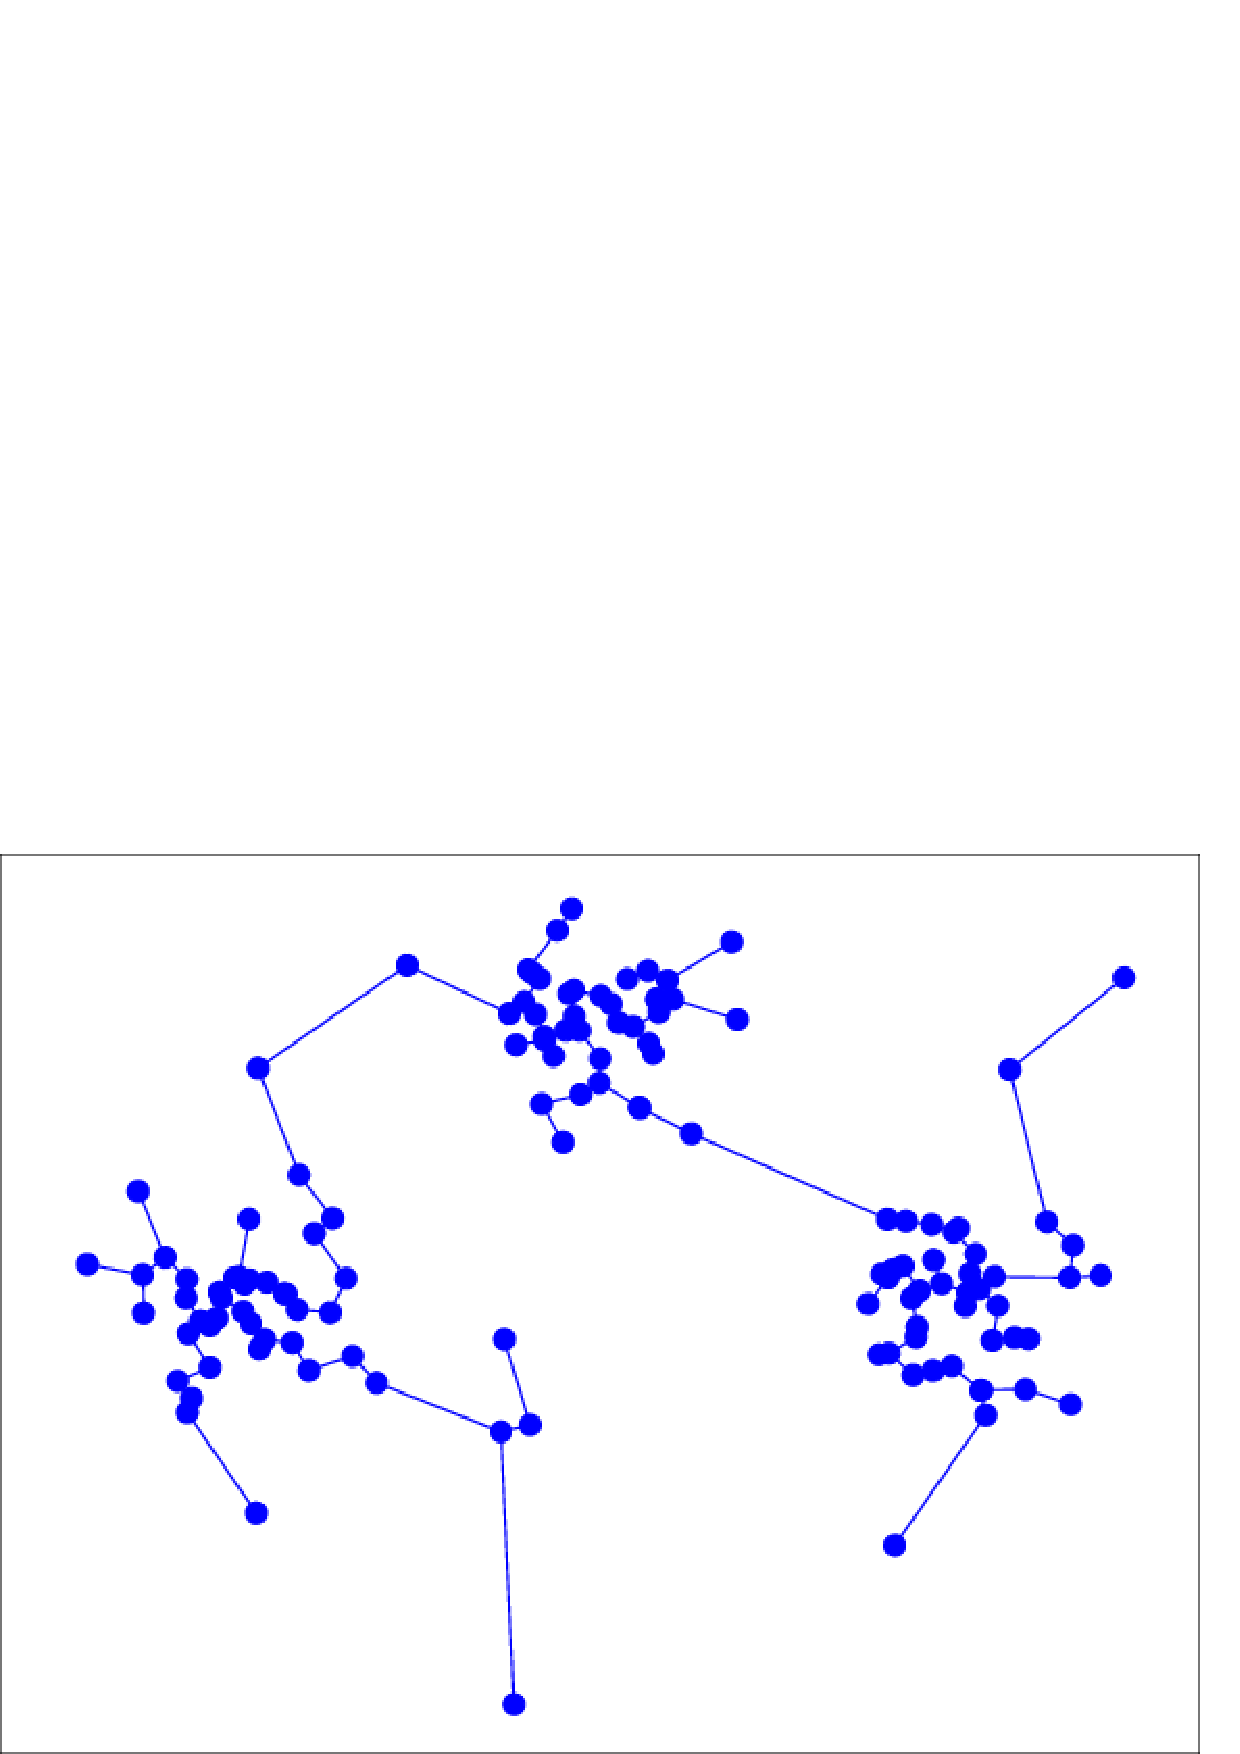
\includegraphics[width=.45\textwidth]{times_MNIST}
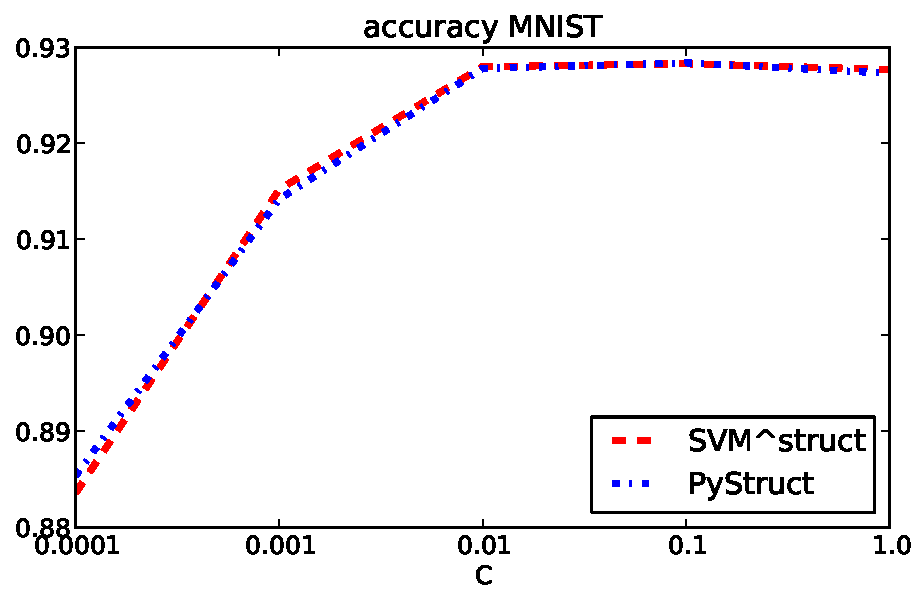
\includegraphics[width=.45\textwidth]{accs_MNIST}
\caption{Runtime comparison of \pystruct and \svmstruct for multi-class
    classification.
}
\label{fig:timings}
\end{figure}

\section{Comparing Learning Algorithms}
%TODO experiments!!

\section{Summary}
%TODO summarize structured prediction
This chapter introduced \pystruct, a modular structured learning and prediction library in Python.
\pystruct is geared towards ease of use, while providing efficient implementations.
\pystruct integrates itself into the scientific Python eco-system, making it easy to use with
existing libraries and applications.
Currently, \pystruct focuses on max-margin and perceptron-based approaches. In the future,
we plan to integrate other paradigms, such as sampling-based learning~\citep{wick2011samplerank},
surrogate objectives (for example pseudo-likelihood), and approaches that allow for a better integration
of inference and learning~\citep{meshi2010learning}.
